\documentclass{article}
\usepackage[T1]{fontenc}
\usepackage{lmodern}
\usepackage{booktabs}
\usepackage{tikz}
\usepackage{hyperref}

\begin{document}
\section{A reproducible workflow}
Table~\ref{tab:checks} records the checks in the process.
Figure~\ref{fig:workflow} shows their order.

\begin{table}[htbp]
  \centering
  \caption{Checks for a small teaching document.}
  \label{tab:checks}
  \begin{tabular}{llr}
    \toprule
    Stage & Check & Count \\
    \midrule
    Source & Main document & 1 \\
    Build & Compilation passes & 2 \\
    Review & Human reading & 1 \\
    \bottomrule
  \end{tabular}
\end{table}

\begin{figure}[htbp]
  \centering
  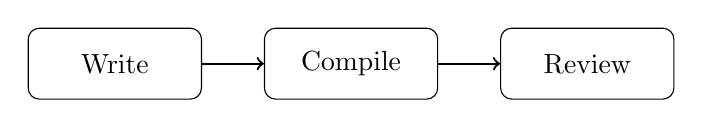
\begin{tikzpicture}[every node/.style={draw,rounded corners,
      minimum width=22mm,minimum height=9mm}]
    \node (write) at (0,0) {Write};
    \node (compile) at (3,0) {Compile};
    \node (review) at (6,0) {Review};
    \draw[->,thick] (write) -- (compile);
    \draw[->,thick] (compile) -- (review);
  \end{tikzpicture}
  \caption{Text description: write the source, compile it, then review the PDF.}
  \label{fig:workflow}
\end{figure}

Float placement is a preference, not an instruction to place an object
at an exact screen coordinate.
\end{document}
